%%% PLOT FILE - Perceptions of the robots - main effect of the robot on warmth and discomfort
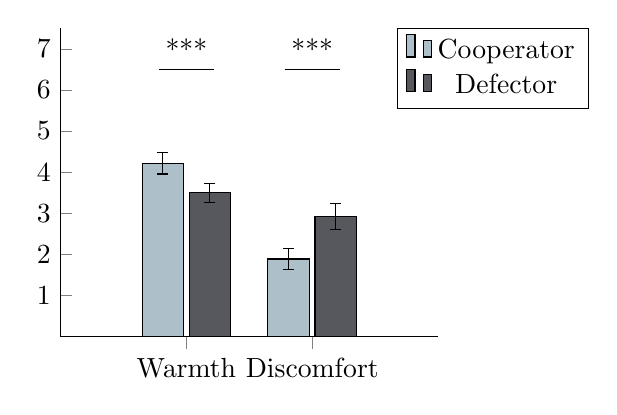
\begin{tikzpicture}%
\begin{axis}[%
    ybar,%
    %title=Test,%
    axis y line*=left, axis x line*=bottom,%
    ymin=0,
    ymax=7.5,
    ytick={1,2,...,7},
    legend style={at={(1.4,1)}},
    %x tick label style={rotate=45,anchor=east},%
    symbolic x coords={Warmth,Discomfort},%
    xtick=data,
    enlarge x limits=1,
    bar width=15pt,
    height=5.5cm,
    %ylabel=difference in \%,%
        ]%
\addplot+[
    color=black, %
    fill={rgb,255:red,173; green,192; blue,202},%
    %postaction={pattern=crosshatch dots},
    error bars, y dir=both, y explicit]
				coordinates {
				(Warmth,4.22) +- (Warmth,0.264)
				(Discomfort,1.89) +- (Discomfort,0.258)};
\addplot+[%
    color=black, %
    fill={rgb,255:red,87; green,87; blue,94},%
    error bars/.cd,%
    y dir=both,%
    y explicit,%
        ]%
coordinates {
            (Warmth,3.50) +- (Warmth,0.236)
            (Discomfort,2.92) +- (Discomfort,0.31)
        };%
    
\draw (axis cs:Warmth,6.5) ++ (-10pt,0pt) -- ++(20pt,0pt);
\node[anchor=south] at (axis cs:Warmth,6.5) {***};
    
\draw (axis cs:Discomfort,6.5) ++ (-10pt,0pt) -- ++(20pt,0pt);
\node[anchor=south] at (axis cs:Discomfort,6.5) {***};

\legend{Cooperator,Defector}
\end{axis}%
\end{tikzpicture}%